%!TEX program = xelatex
\documentclass[a4paper,11pt]{article}
\usepackage{kotex}
\usepackage{amsmath,amssymb}
\usepackage{geometry}
\usepackage{multicol}
\usepackage{array}
\usepackage{enumitem}
\usepackage{tikz}
\usepackage{xcolor}
\usepackage{mdframed}

\geometry{top=15mm, bottom=15mm, left=15mm, right=15mm}

\setmainfont{NanumMyeongjo}
\setsansfont{NanumGothic}

\setlength{\columnseprule}{0.4pt}
\setlength{\columnsep}{8mm}

\newcommand{\choicenum}[1]{\textcircled{\small #1}}
\newcommand{\scorebox}[1]{\textbf{(#1점)}}
\newcommand{\qbox}[1]{%
  \begin{mdframed}[linewidth=0.8pt,innerleftmargin=6pt,innerrightmargin=6pt,innertopmargin=4pt,innerbottommargin=4pt]
  #1
  \end{mdframed}
}

\pagestyle{empty}

\begin{document}

%--- 헤더 ---
\begin{center}
{\large \textbf{3학년 1학기 중간고사 \quad 수학 \quad [B형]}}\\[2pt]
{\normalsize 선택형 1번\,--\,16번 \;/\; 서술형 1번\,--\,8번 \quad 총 4쪽}
\end{center}
\vspace{1mm}
\hrule height 1pt
\vspace{3mm}

\begin{multicols}{2}

%===========================================================
%  선택형
%===========================================================

\noindent\textbf{1.} $\sqrt{(-7)^{2}}$의 제곱근은? \scorebox{3}

\begin{enumerate}[label=\protect\choicenum{\arabic*},leftmargin=*,itemsep=0pt]
  \item $\pm\,7$
  \item $\pm\,\sqrt{7}$
  \item $7$
  \item $-7$
  \item $49$
\end{enumerate}

\vspace{3mm}

\noindent\textbf{2.} 실수의 대소관계로 옳은 것은? \scorebox{3}

\begin{enumerate}[label=\protect\choicenum{\arabic*},leftmargin=*,itemsep=0pt]
  \item $\sqrt{10} > 4$
  \item $\sqrt{3} < 1$
  \item $-\sqrt{10} > -3$
  \item $-\sqrt{26} < -5$
  \item $\dfrac{\sqrt{2}}{3} > \dfrac{\sqrt{3}}{3}$
\end{enumerate}

\vspace{3mm}

\noindent\textbf{3.} 다음을 계산하면? \scorebox{3}

\qbox{$\sqrt{50} \div \sqrt{2} \times 3\sqrt{5}$}

\begin{enumerate}[label=\protect\choicenum{\arabic*},leftmargin=*,itemsep=0pt]
  \item $3\sqrt{5}$
  \item $9\sqrt{5}$
  \item $15\sqrt{5}$
  \item $18\sqrt{5}$
  \item $45\sqrt{5}$
\end{enumerate}

\vspace{3mm}

\noindent\textbf{4.} 다음 식을 전개하면? \scorebox{3}

\qbox{$(4x+3y)(4x-3y)$}

\begin{enumerate}[label=\protect\choicenum{\arabic*},leftmargin=*,itemsep=0pt]
  \item $4x^{2}-3y^{2}$
  \item $16x^{2}-9y^{2}$
  \item $16x^{2}+9y^{2}$
  \item $16x^{2}+24xy-9y^{2}$
  \item $16x^{2}-24xy+9y^{2}$
\end{enumerate}

\vspace{3mm}

\noindent\textbf{5.} 다음 식이 완전제곱식이 되도록\\
\quad $\square$ 안에 알맞은 수를 고르면? \scorebox{3}

\qbox{$9x^{2}+\square\,x+4$}

\begin{enumerate}[label=\protect\choicenum{\arabic*},leftmargin=*,itemsep=0pt]
  \item $6$
  \item $9$
  \item $12$
  \item $18$
  \item $36$
\end{enumerate}

\vspace{3mm}

\noindent\textbf{6.} 다음 이차방정식을 풀면? \scorebox{3}

\qbox{$x^{2}-5x=0$}

\begin{enumerate}[label=\protect\choicenum{\arabic*},leftmargin=*,itemsep=0pt]
  \item $x=0$
  \item $x=5$
  \item $x=0$ 또는 $x=-5$
  \item $x=0$ 또는 $x=5$
  \item $x=-5$ 또는 $x=5$
\end{enumerate}

\vspace{3mm}

\noindent\textbf{7.} 무리수만으로 짝지어진 것을 고르면? \scorebox{4}

\begin{enumerate}[label=\protect\choicenum{\arabic*},leftmargin=*,itemsep=0pt]
  \item $\sqrt{4},\,\sqrt{8},\,\sqrt{16}$
  \item $\sqrt{\dfrac{9}{16}},\,\sqrt{1.21},\,\pi$
  \item $0.5,\,\dfrac{9}{4},\,\sqrt{9}$
  \item $3\sqrt{2},\,5\sqrt{7},\,-\sqrt{0.36}$
  \item $\sqrt{2.25},\,-\sqrt{(-5)^{2}},\,\sqrt{25}-2$
\end{enumerate}

\vspace{3mm}

\noindent\textbf{8.} $1<x<4$일 때, 가장 큰 것을 고르면? \scorebox{4}

\begin{enumerate}[label=\protect\choicenum{\arabic*},leftmargin=*,itemsep=0pt]
  \item $\sqrt{x}$
  \item $x$
  \item $x^{2}$
  \item $\dfrac{4}{x}$
  \item $\dfrac{x}{2}$
\end{enumerate}

\vspace{3mm}

\noindent\textbf{9.} 다음을 계산하면? \scorebox{4}

\qbox{$\sqrt{50}-\sqrt{32}+\sqrt{72}$}

\begin{enumerate}[label=\protect\choicenum{\arabic*},leftmargin=*,itemsep=0pt]
  \item $3\sqrt{2}$
  \item $4\sqrt{2}$
  \item $5\sqrt{2}$
  \item $6\sqrt{2}$
  \item $7\sqrt{2}$
\end{enumerate}

\vspace{3mm}

\noindent\textbf{10.} $\sqrt{8}\!\left(\dfrac{\sqrt{2}}{4}-\sqrt{2}\right)+\dfrac{a}{\sqrt{2}}\!\left(\sqrt{32}-4\right)$이\\
유리수일 때, 유리수 $a$의 값을 구하면? \scorebox{4}

\begin{enumerate}[label=\protect\choicenum{\arabic*},leftmargin=*,itemsep=0pt]
  \item $\dfrac{1}{2}$
  \item $1$
  \item $\dfrac{3}{2}$
  \item $2$
  \item $-1$
\end{enumerate}

\vspace{3mm}

\noindent\textbf{11.} 식을 전개할 때, $x$의 계수가 다른 하나는? \scorebox{4}

\begin{enumerate}[label=\protect\choicenum{\arabic*},leftmargin=*,itemsep=0pt]
  \item $(x+2)(x-7)$
  \item $(x+5)(-x+4)$
  \item $(x+3)(2x-5)$
  \item $(2x+3)(3x-2)$
  \item $(2x+7)(2x-3)$
\end{enumerate}

\vspace{3mm}

\noindent\textbf{12.} 다음 식을 전개하면? \scorebox{4}

\qbox{$(2x+5y)^{2}-16\!\left(\dfrac{1}{2}x+y\right)^{2}$}

\begin{enumerate}[label=\protect\choicenum{\arabic*},leftmargin=*,itemsep=0pt]
  \item $-4xy-9y^{2}$
  \item $4xy+21y^{2}$
  \item $4x^{2}+12xy+9y^{2}$
  \item $-2xy+7y^{2}$
  \item $4x^{2}+28xy+21y^{2}$
\end{enumerate}

\vspace{3mm}

\noindent\textbf{13.} 다음 두 다항식을 인수분해 할 때, 공통으로 들어 있는 인수는? \scorebox{4}

\qbox{$-(x-4)+3x(x-4),\quad 6x^{2}-7x-3$}

\begin{enumerate}[label=\protect\choicenum{\arabic*},leftmargin=*,itemsep=0pt]
  \item $x-4$
  \item $3x-1$
  \item $3x+1$
  \item $2x-3$
  \item $2x+3$
\end{enumerate}

\vspace{3mm}

\noindent\textbf{14.} 다음 그림과 같은 직사각형의 빗금친 부분의 넓이를 구하면? \scorebox{4}

\begin{center}
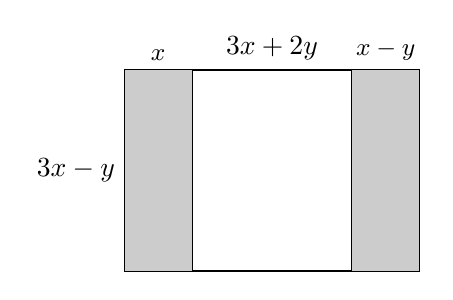
\begin{tikzpicture}[scale=0.85]
  \draw[thick] (0,0) rectangle (4.4,3.0);
  \draw[thick] (1.0,0) rectangle (3.4,3.0);
  \fill[gray!40] (0,0) rectangle (1.0,3.0);
  \fill[gray!40] (3.4,0) rectangle (4.4,3.0);
  \node[above] at (2.2,3.0) {$3x+2y$};
  \node[above] at (0.5,3.0) {\small $x$};
  \node[above] at (3.9,3.0) {\small $x-y$};
  \node[left] at (0,1.5) {$3x-y$};
\end{tikzpicture}
\end{center}

\begin{enumerate}[label=\protect\choicenum{\arabic*},leftmargin=*,itemsep=0pt]
  \item $5x^{2}-6xy-y^{2}$
  \item $6x^{2}-6xy+y^{2}$
  \item $6x^{2}-9xy-y^{2}$
  \item $8x^{2}-6xy+y^{2}$
  \item $9x^{2}-6xy-y^{2}$
\end{enumerate}

\vspace{3mm}

\noindent\textbf{15.} $-\dfrac{1}{2}<x<3$일 때, 다음 식을 간단히 하면? \scorebox{5}

\qbox{$\sqrt{4x^{2}+4x+1}-\sqrt{x^{2}-6x+9}$}

\begin{enumerate}[label=\protect\choicenum{\arabic*},leftmargin=*,itemsep=0pt]
  \item $-x-4$
  \item $x+4$
  \item $-x+2$
  \item $x-2$
  \item $3x-2$
\end{enumerate}

\vspace{3mm}

\noindent\textbf{16.} 두 자연수 $a,\,b$에 대하여 다항식 $2x^{2}+9x+k$가\\
$(2x+a)(x+b)$로 인수분해 되도록 하는 실수 $k$의\\
최댓값은? \scorebox{5}

\begin{enumerate}[label=\protect\choicenum{\arabic*},leftmargin=*,itemsep=0pt]
  \item $4$
  \item $9$
  \item $10$
  \item $18$
  \item $20$
\end{enumerate}

\end{multicols}

\newpage

%===========================================================
%  서술형
%===========================================================
\begin{center}
{\large \textbf{서술형 \quad [B형]}}
\end{center}
\noindent{\small ※ 서술형 문항은 \textbf{서술형 답지}에 풀이과정과 답을 쓰고 제출해야 합니다.}
\vspace{4mm}
\hrule
\vspace{4mm}

\begin{enumerate}[leftmargin=*,itemsep=10mm]

\item[\textbf{서술형 1.}] $\dfrac{\sqrt{3}-2}{\sqrt{3}}$의 분모를 유리화하여라. \scorebox{4}

\vspace{30mm}

\item[\textbf{서술형 2.}] 다음 식을 전개하여라. \scorebox{4}

\qbox{$(3x+2)^{2}-4x(x+1)$}

\vspace{35mm}

\item[\textbf{서술형 3.}] 다음 이차방정식을 인수분해를 이용하여 풀어라. \scorebox{5}

\qbox{$2x^{2}+x-15=0$}

\vspace{35mm}

\item[\textbf{서술형 4.}] $\sqrt{\dfrac{540}{x}}$이 자연수가 되도록 하는 자연수 $x$의 값을 모두 구하여라. \scorebox{5}

\vspace{35mm}

\item[\textbf{서술형 5.}] 이차식 $ax^{2}-7x+3$, $2x^{2}+bx-6$의\\
공통인수가 $x-3$일 때, $a+b$의 값을 구하여라. \scorebox{5}

\vspace{35mm}

\item[\textbf{서술형 6.}] $3^{2}-5^{2}+7^{2}-9^{2}+11^{2}-13^{2}$을\\
인수분해를 이용하여 계산하여라. \scorebox{5}

\vspace{35mm}

\item[\textbf{서술형 7.}] 다음 두 부등식을 모두 만족시키는 자연수 $x$의\\
값을 모두 더하면? \scorebox{6}

\qbox{%
\begin{tabular}{l}
① $\sqrt{8} < \sqrt{x} < \sqrt{30}$ \\[4pt]
② $-4 < -\sqrt{x} < -2$
\end{tabular}
}

\vspace{40mm}

\item[\textbf{서술형 8.}] 사다리꼴 $PQRS$의 넓이를 구하고, 이것이\\
직사각형 $ABCD$의 넓이의 몇 배인지 구하여라. \scorebox{6}

\begin{center}
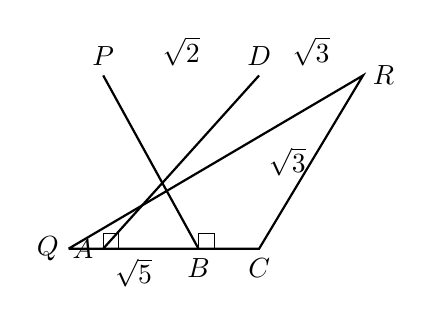
\begin{tikzpicture}[scale=1.1]
  \coordinate (Q) at (0,0);
  \coordinate (B) at (1.5,0);
  \coordinate (C) at (2.2,0);
  \coordinate (P) at (0.4,2.0);
  \coordinate (R) at (3.4,2.0);
  \coordinate (A) at (0.4,0);
  \coordinate (D) at (2.2,2.0);
  \draw[thick] (Q)--(R)--(C)--(Q);
  \draw[thick] (A)--(D);
  \draw[thick] (B)--(P);
  \draw (A) rectangle ++(0.18,0.18);
  \draw (B) rectangle ++(0.18,0.18);
  \node[left] at (Q) {$Q$};
  \node[below] at (B) {$B$};
  \node[below] at (C) {$C$};
  \node[above] at (P) {$P$};
  \node[right] at (R) {$R$};
  \node[above] at (D) {$D$};
  \node[left] at (A) {$A$};
  \node[below] at (0.75,0) {$\sqrt{5}$};
  \node[right] at (2.2,1.0) {$\sqrt{3}$};
  \node[above] at (1.3,2.0) {$\sqrt{2}$};
  \node[above] at (2.8,2.0) {$\sqrt{3}$};
\end{tikzpicture}
\end{center}

\end{enumerate}

\end{document}
